\section{Introduction}
\label{sec:introduction}
Embedded robots run perception, localization, mapping, planning, and control
on shared compute resources. Platforms with CPUs, GPUs, and dedicated neural
accelerators offer several places to run a detector. Using an accelerator
requires checking which parts of the detector actually run on it.

Nominal DLA deployment differs from verified fallback-free placement of the
learned graph. TensorRT can request DLA execution while allowing unsupported
regions to run on GPU \cite{nvidia_dla_working}. Operator support, tensor shapes,
normalization axes, precision, and I/O layouts constrain placement. A successful
export or a DLA build option alone cannot show where the learned layers execute.

The question is what full DLA placement of a modern detector costs, and where
that cost falls. YOLO11
\cite{jocher2024yolo11} serves as the case study. Its architecture combines a convolutional backbone and neck with spatial self-attention and a decoded prediction interface.
These expose two parts of the deployment problem: incompatible learned
operations and the boundary between the accelerator graph and detection processing.

\begin{figure}[t]
    \centering
    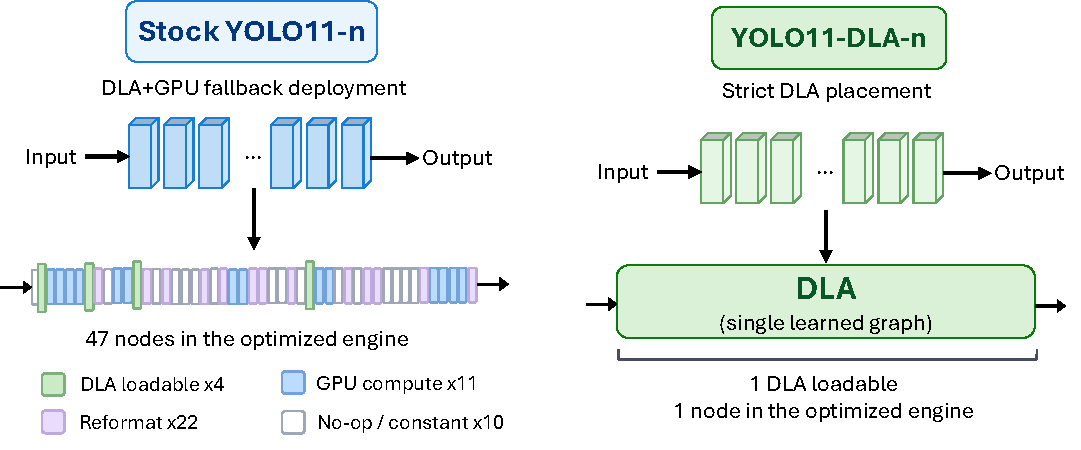
\includegraphics[width=\columnwidth]{figures/teaser.pdf}
    \caption{FP16 deployment. Stock YOLO11-n uses DLA+GPU fallback;
    YOLO11-DLA-n places the complete learned graph in one DLA loadable.
    Host-side decoding and non-maximum suppression remain outside the accelerator.}
    \label{fig:teaser}
\end{figure}

The workflow starts by inspecting the detector and its exported graph, then
attempting strict DLA compilation. The strict compilation failure identifies the blocking learned computation, while the desired accelerator boundary guides the output-interface change. In YOLO11, the attention block forms a spatial affinity matrix through a query--key MatMul that strict DLA compilation rejects. The stock detection head also performs DFL expectation, grid decoding, sigmoid, flattening, and cross-scale concatenation inside the exported graph. Section~\ref{sec:method} replaces the incompatible attention computation with C2DLA and moves the prediction boundary earlier through DetectDLA, which exports three static raw prediction maps. The adapted graph is then compiled with GPU fallback disabled,
and the optimized engine is inspected (Fig.~\ref{fig:teaser}). Host-side decoding,
confidence filtering, and non-maximum suppression (NMS) complete the detector.
The resulting nano model is denoted \model.
The anonymous model implementation is available at \url{https://anonymous.4open.science/r/ultralytics-dla}; the export, deployment, benchmarking, evaluation code, and trained weights are available at \url{https://anonymous.4open.science/r/yolo11_dla}.

\begin{figure*}[t]
\centering
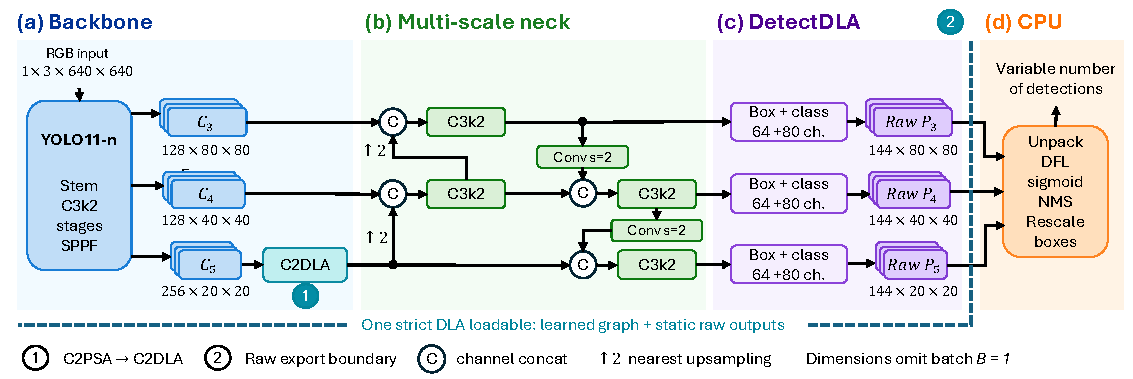
\includegraphics[width=\textwidth]{figures/architecture_overview.pdf}
\caption{\textbf{YOLO11-DLA-n architecture.} Backbone scales feed the neck and box/class
 towers at strides 8, 16, and 32. Markers 1 and 2 identify C2DLA and the raw-output
 boundary. The learned graph forms one DLA loadable; unpacking and post-processing
 remain on CPU. Preprocessing and input packing precede the graph.}
\label{fig:boundary}
\end{figure*}

This work makes three contributions:
\begin{itemize}
\item A modern detector made fully DLA-admissible still runs as one DLA
loadable with no GPU-assigned learned layer, in FP16 and in INT8: fallback-disabled
compilation and optimized-engine inspection verify the placement, which C2DLA
and DetectDLA obtain while retaining the surrounding backbone, neck, detection
towers, and training formulation.
\item The accuracy cost of full placement is negligible in FP16 and non-zero in
INT8. Strict DLA scores $-0.003$ AP in FP16 and $-0.543$ AP in INT8 against the
same network on GPU: the precision regime, not the placement, dominates the
accuracy loss.
\item Latency and energy reverse at the application boundary, and the cause is
measured. In INT8 the inference stage is faster on strict DLA than on the adapted
GPU engine (4.522 versus 6.400\,ms), while the native-layout input and output
boundaries have stage medians of 7.463 and 10.729\,ms, and the adapted GPU configuration remains
faster and lower-energy over the whole pipeline.
\end{itemize}

Moving the learned detector away from GPU compute motivates this study, but concurrent workloads are not evaluated. The evidence here covers the YOLO11 case study on the tested
Orin/TensorRT configuration.
